\documentclass[pdftex]{article}
\usepackage[pdftex]{graphics}
\usepackage{subfigure}
\usepackage{hhline}
\usepackage[usenames,dvipsnames]{color}
\usepackage{colortbl}
\usepackage[screen,pdftex]{mcdlecture}
\newcommand{\bs}{\relax}
\newcommand{\es}{\newpage}
\fboxsep=.01\textwidth \fboxrule=1pt
\newsavebox{\savepar}
\newenvironment{boxit}{\begin{lrbox}{\savepar}
    \begin{minipage}[b]{0.975\textwidth}}
    {\end{minipage}\end{lrbox}\framebox{\usebox{\savepar}}}


%%%%%%%%%%%%%%%%%%%%%%%%%%%%%%%%%%%%%%%%%%%%%%%%%%%%%%%%%%
%% THE FOLLOWING ARE THINGS THAT WE MIGHT CHANGE FROM YEAR TO YEAR OR
%% VENUE TO VENUE
    \lhead{MCMC in Statistical Genetics}
    \lfoot{Dr Eric C. Anderson and Dr Matthew Stephens}
%	\lfoot{Dr Eric C. Anderson and Dr John Novembre}
%    \rfoot{UW - Summer Institute, July 2013}
%	 \rfoot{Edinburgh - European Institute, June 2012}
\rfoot{Brazil - Summer Institute, February 2014}

% on this one, be sure to update the venue and the module number
%\newcommand{\coursetitlepage}{European Institute in Statistical Genetics
%\newcommand{\coursetitlepage}{Summer Institute in Statistical Genetics
\newcommand{\coursetitlepage}{Brazilian Edition of the Summer \\Institute in Statistical Genetics

Module 9:

MCMC for Genetics}

%% Then update the schedule.  Note that I have broken that
%% out into a separate file like: schedule_table_edinburgh2012.tex
%% which is input in Overview.tex

%% Then be sure to change any time-sensitive events in the 
%% probability discussion in Matthew's first lecture.

%% And also update "structure_fun" link to my wiki to the right
%% year and venue.
%%%%%%%%%%%%%%%%%%%%%%%%%%%%%%%%%%%%%%%%%%%%%%%%%%%%%%%%%%


\begin{document}

\DeclareGraphicsExtensions{.jpg,.pdf,.png}%



%% Eric added a few things:
% some commands that Eric made for making a title while starting
% a new lecture and for making titles of new slides.
\newcommand{\newlecture}[1]{\newpage\begin{center}\section*{#1}\end{center}}
\newcommand{\newslide}[1]{\newpage\subsection*{#1: \hfil}}
 \newcommand{\Exp}{\Bbb{E}}
 \newcommand{\Var}{{\mathrm{Var}}}
 %% Some pretty etc.'s, etc...
\newcommand{\cf}{{\em cf.}}
\newcommand{\eg}{{\em e.g.},}
\newcommand{\ie}{{\em i.e.},}
\newcommand{\etal}{{\em et al.}\ }
\newcommand{\etc}{{\em etc.}}

%% some handy things for making bold math
\def\bm#1{\mathpalette\bmstyle{#1}}
\def\bmstyle#1#2{\mbox{\boldmath$#1#2$}}
\newcommand{\thh}{^\mathrm{th}}
\newcommand{\bpi}{{\pi}}
\newcommand{\mP}{\mathbf{P}}
\rhead{Session 3 - \thepage}


\small
\begin{verbatim}

# Session 3: Introduction to MCMC in R (Computing Practical)
# 
# Note: anything following a # sign is a comment, and will be ignored by R
# (this should make it easier to cut and paste things)
#
#
# Example 1: sampling from an exponential distribution using MCMC
#
# 
# first: a few example lines of R

R
x = seq(from = 0, to = 10, length=20)
?seq    # to get help on any command in R you can type ?command
x       # to see what an object looks like, just type its name
y = exp(-x)
y       # note that y is a vector, because x is a vector
plot(x,y)
lines(x,y) #lines adds lines to an existing plot

#
# We will learn more R as we go along: ask questions if there is
# something you don't understand!
#
# Now: set up a target function we want to sample from
# In this case we are going to use the density of the exponential distribution
# (What follows is not the best way to do things, but I have tried
# to make it easy to follow for novice users)
#

target = function(x){
if(x<0){
return(0)}
else {
return( exp(-x))
}
}

#Try computing a couple of values

target(1)
target(-1)
\end{verbatim}

\es\bs

\begin{verbatim}

# Next, we will program a Metropolis--Hastings scheme to sample
# from a distribution proportional to the target

x = rep(0,1000)
x[1] = 3     #this is just a starting value, which I've set arbitrarily to 3
for(i in 2:1000){
currentx = x[i-1]
proposedx = currentx + rnorm(1,mean=0,sd=1)
A = target(proposedx)/target(currentx) 
if(runif(1)<A){
x[i] = proposedx       # accept move with probabily min(1,A)
} else {
x[i] = currentx        # otherwise "reject" move, and stay where we are
}
}

# note that x is a realisation of a Markov Chain
# we can make a few plots of x:
plot(x) 
hist(x)

\end{verbatim}
\es\bs

\begin{verbatim}
# We can wrap this up in a function to make things a bit neater,
# and make it easy to try changing starting values and proposal distributions


easyMCMC = function(niter, startval, proposalsd){
x = rep(0,niter)
x[1] = startval     
for(i in 2:niter){
currentx = x[i-1]
proposedx = rnorm(1,mean=currentx,sd=proposalsd) 
A = target(proposedx)/target(currentx)
if(runif(1)<A){
x[i] = proposedx       # accept move with probabily min(1,A)
} else {
x[i] = currentx        # otherwise "reject" move, and stay where we are
}
}
return(x)
}
\end{verbatim}
\es\bs

\begin{verbatim}
#Now we'll run the MCMC scheme 3 times, 
#and look to see how similar the results are


z1=easyMCMC(1000,3,1)
z2=easyMCMC(1000,3,1)
z3=easyMCMC(1000,3,1)

plot(z1,type="l")
lines(z2,col=2)
lines(z3,col=3)


par(mfcol=c(3,1)) #rather odd command tells R to put 3 graphs on a single page
hist(z1)
hist(z2)
hist(z3)

\end{verbatim}
\es\bs

\begin{verbatim}
# Exercises: use the function easyMCMC to explore the following:
#
# 1a) how do different starting values affect the MCMC scheme?  
#
# 1b) what is the effect of having a bigger/smaller proposal standard deviation?
#
# 1c) try changing the target function to the following
#

target = function(x){
return((x>0 & x <1) + (x>2 & x<3))
}

# What does this target look like?
# What happens if the proposal sd is too small here? (try eg 1 and 0.1)

\end{verbatim}
\es\bs


\section*{\hfil MCMC Convergence \hfil}

Markov chain Monte Carlo relies on the fact that, asymptotically (i.e. after
infinite iterations),
simulated values from the Markov chain behave as if they were
sampled from the joint posterior distribution we are interested
in.

In practice we can't perform infinitely many iterations before we
regard the simulated values as coming from the posterior
distribution. Thus we hope that provided we do enough iterations our
simulated values will be sufficiently close to coming from the
posterior distribution. But how do we know when we are
sufficiently close?

\es\bs
\section*{Assessing Convergence}

Although ``formal'' methods exist for assessing convergence,
I tend to prefer less formal methods.

Here are some guidelines for assessing problems:
\begin{itemize}
   \item Always run the MCMC sampler multiple times from different starting points.
   \item Compare results from different starting points: do they differ enough to change your conclusions?
   \item Plot trace plots of different parameters against iteration number: do they look ``sticky?''
   \end{itemize}
   

\es\bs
\section*{Improving Convergence}

If convergence appears to be a problem, you can try:
\begin{itemize}
   \item Running the sampler longer!
   \item Changing the model (convergence problems tend to occur more often when the model is wrong).
   \item Tuning the MH proposal standard deviation.
   \item Redesigning the sampler.
   \end{itemize}
   
   In some difficult problems, getting a sampler to converge is very difficult. In these cases
   MCMC can sometimes still provide useful output, if started from a ``good'' starting point.
Think of it as a local exploration of a ``good" solution.   
   
\es\bs
\section*{Example: A bimodal target}

\centerline{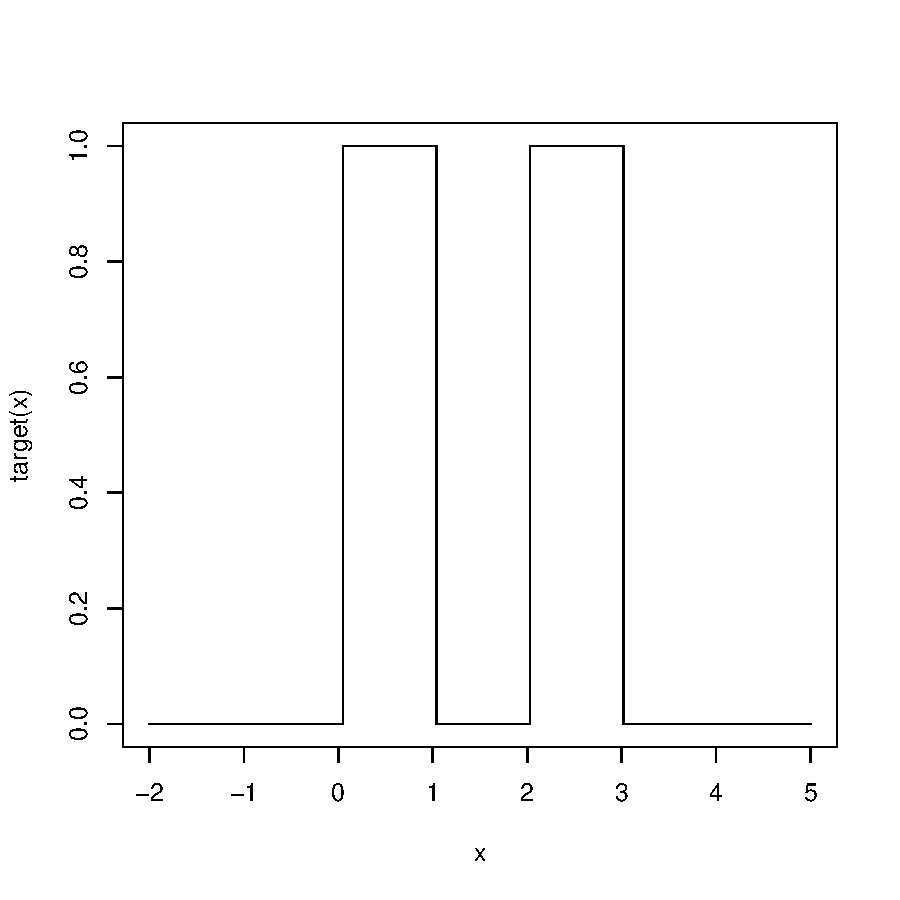
\includegraphics[height=4.5in]{figures/target.pdf}}

\es\bs

\section*{SD = 1 gives satisfactory results}
\centerline{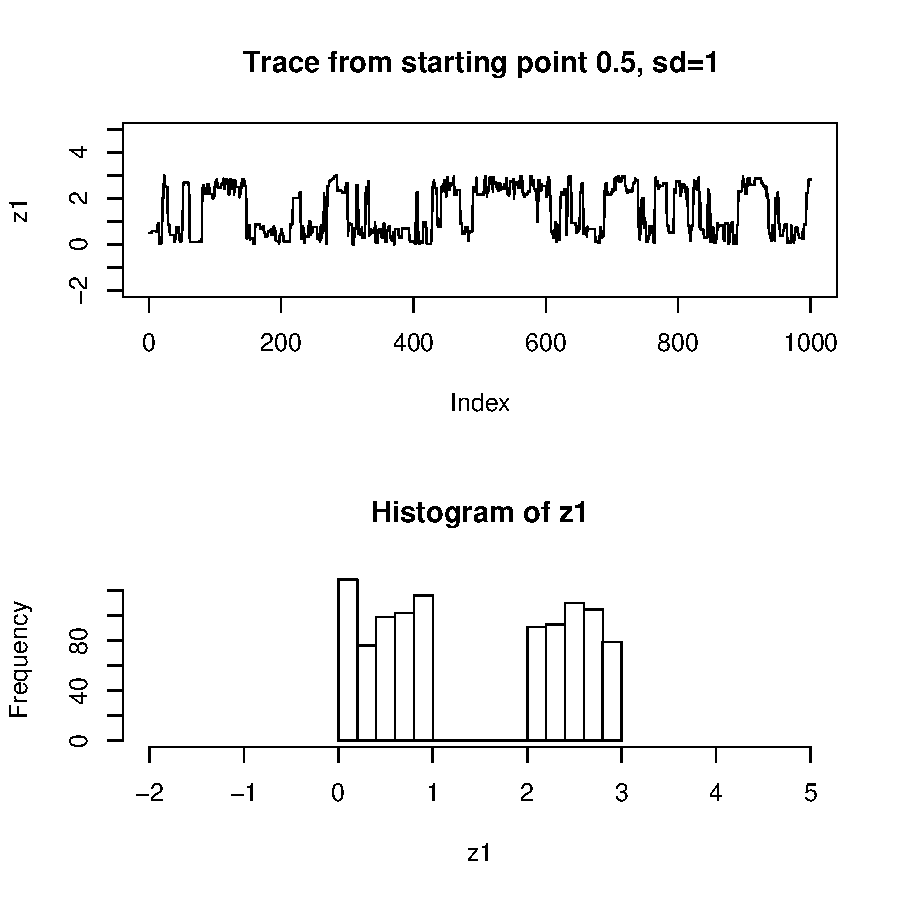
\includegraphics[height=4.5in]{figures/goodtrace1.pdf}}
\es\bs

\section*{SD = 1: different starting points agree well}
\centerline{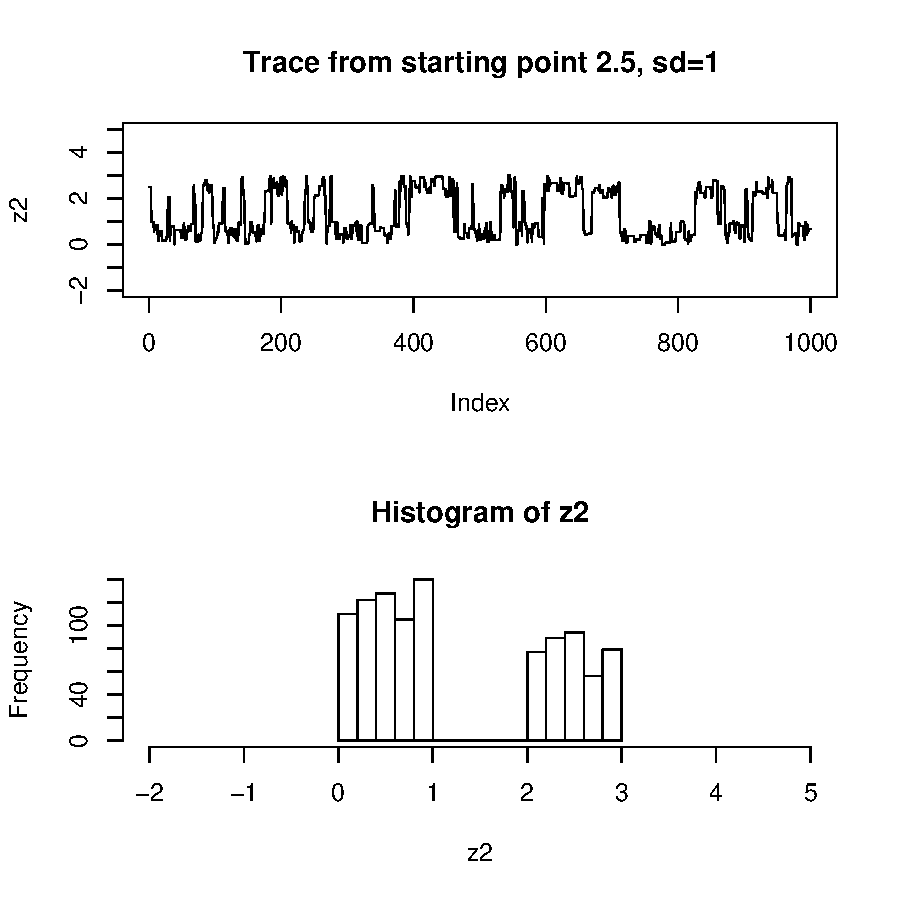
\includegraphics[height=4.5in]{figures/goodtrace2.pdf}}

\es\bs
\section*{SD = 1: different starting points agree well}
\centerline{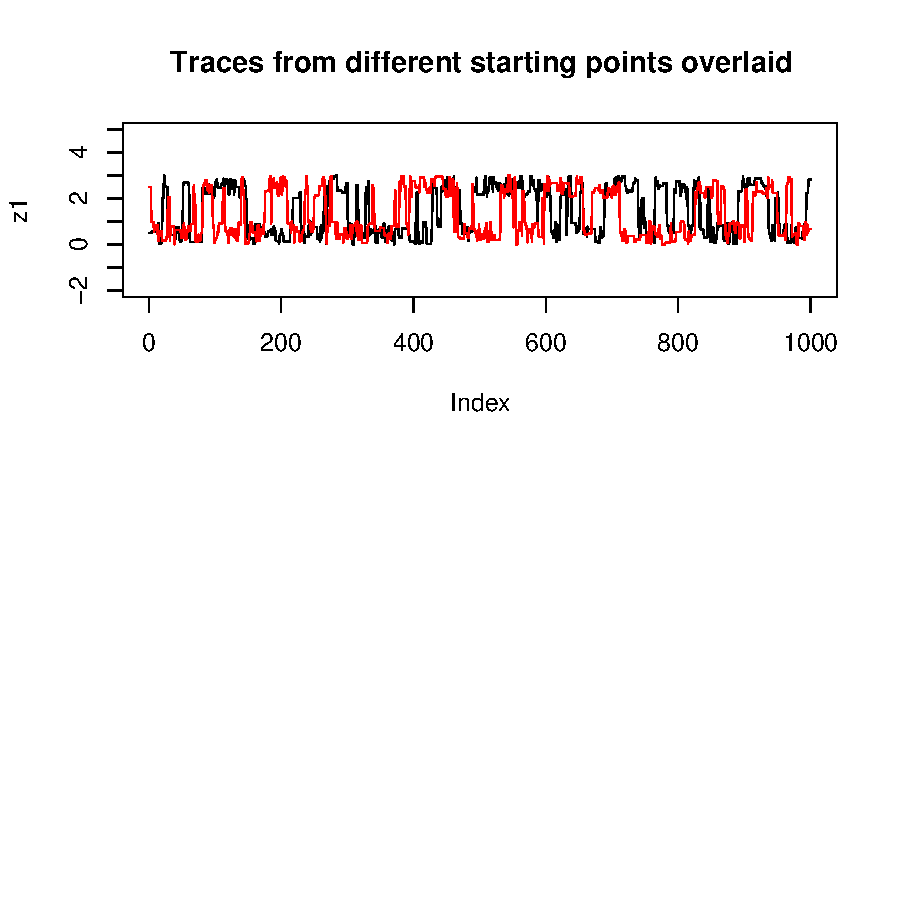
\includegraphics[height=4.5in]{figures/goodtrace3.pdf}}

\es\bs

\section*{SD = 0.1 gives unsatisfactory results}
\centerline{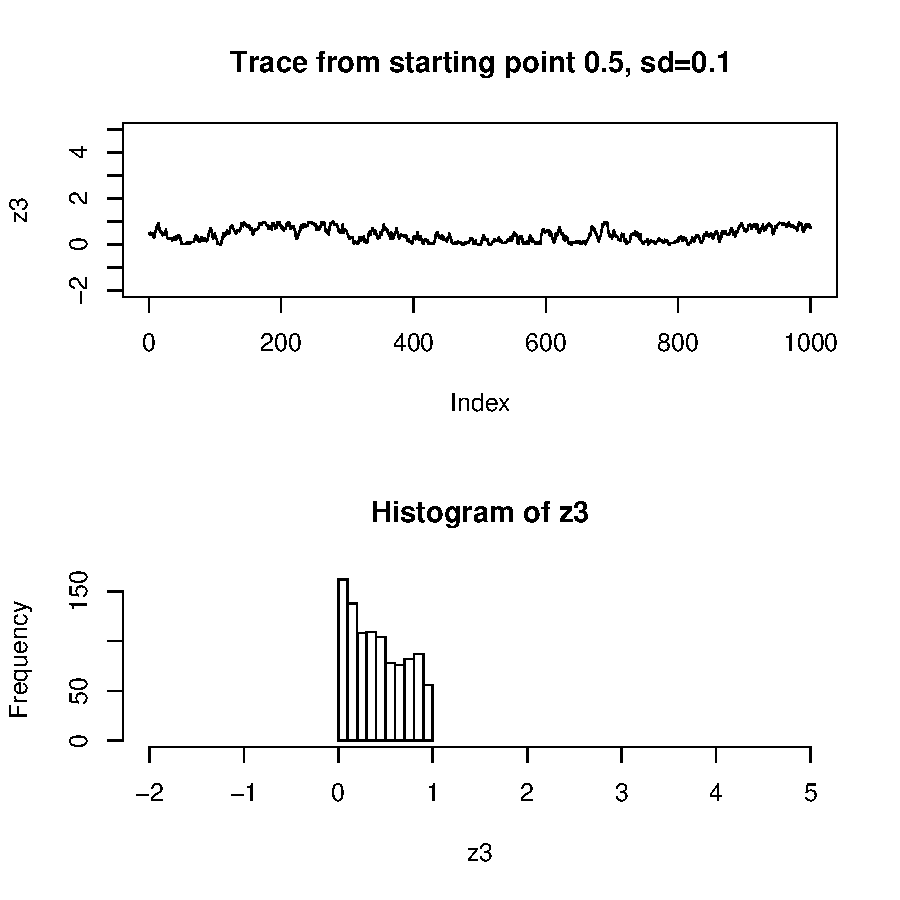
\includegraphics[height=4.5in]{figures/badtrace1.pdf}}
\es\bs

\section*{SD = 0.1: different starting points disagree}
\centerline{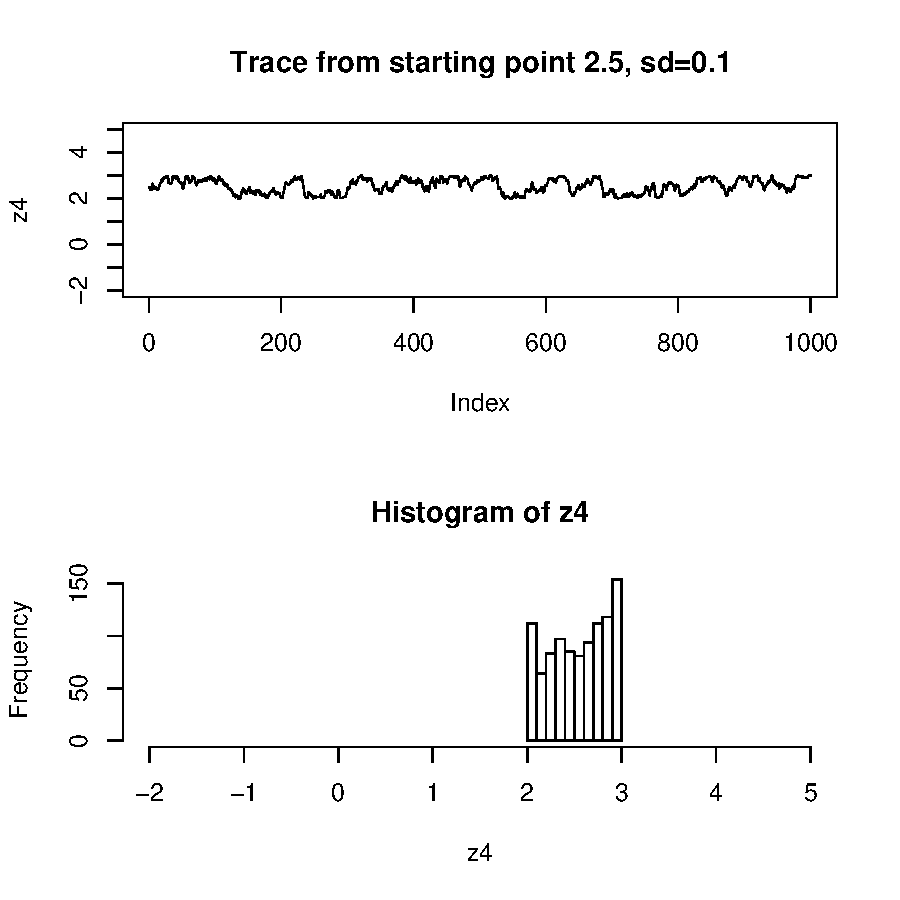
\includegraphics[height=4.5in]{figures/badtrace2.pdf}}

\es\bs
\section*{SD = 0.1: different starting points disagree}
\centerline{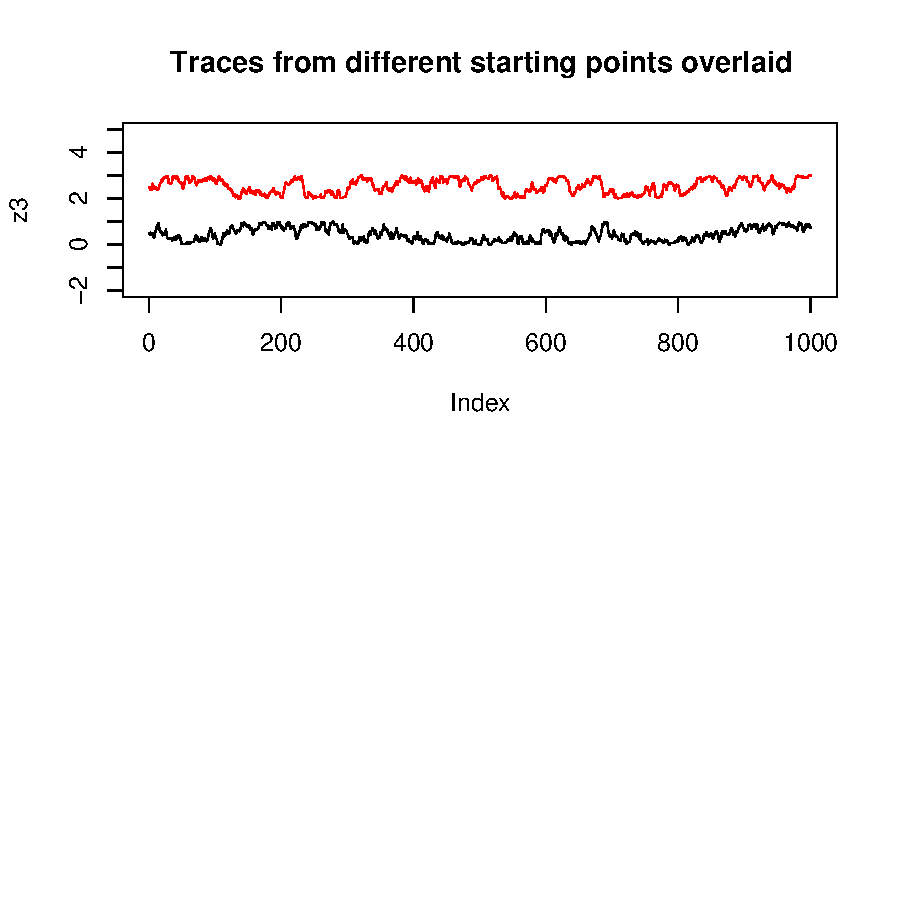
\includegraphics[height=4.5in]{figures/badtrace3.pdf}}

\es\bs

\section*{``Stickiness" of chain depends on SD}
\centerline{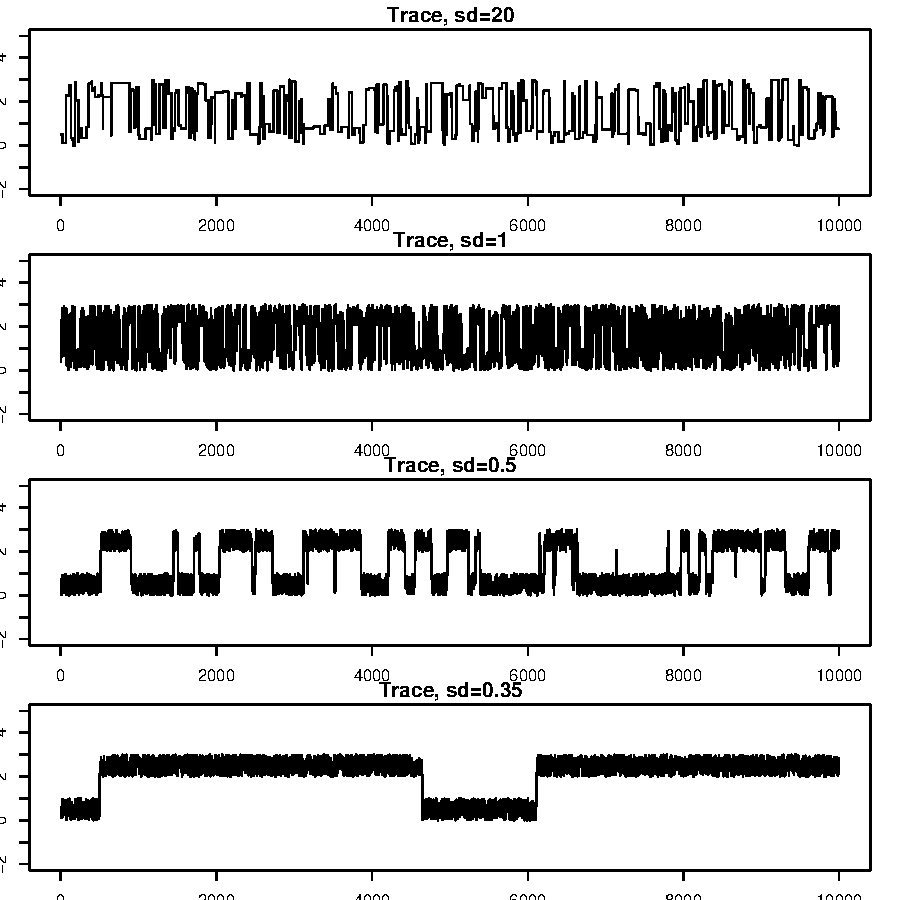
\includegraphics[height=4.5in]{figures/compsd.pdf}}


\es\bs


\begin{verbatim}

# Example 2: Estimating an allele frequency
#
# A standard assumption when modelling genotypes of
# bi-allelic loci (eg loci with alleles A and a) is
# that the population is "randomly mating". From this assumption
# it follows that the population will be in 
# "Hardy Weinberg Equilibrium" (HWE), which means that 
# if p is the frequency of the allele A then the
# genotypes AA, Aa and aa will have frequencies
# p*p, 2p(1-p) and (1-p)*(1-p)
#
# A simple prior for p is to assume it is uniform on [0,1].
# Suppose that we sample n individuals, and observe nAA with genotype AA,
# nAa with genotype Aa and naa with genotype aa. 

# The following R code gives a short MCMC routine to sample from the posterior
# distribution of p. Try to go through the code to see how it works.

prior = function(p){
if((p<0) || (p>1)){  # || here means "or"
return(0)}
else{
return(1)}
}

likelihood = function(p, nAA, nAa, naa){
return(p^(2*nAA) * (2*p*(1-p))^nAa * (1-p)^(2*naa))
}

psampler = function(nAA, nAa, naa, niter, pstartval, pproposalsd){
p = rep(0,niter)
p[1] = pstartval
for(i in 2:niter){
currentp = p[i-1]
newp = currentp + rnorm(1,0,pproposalsd)
A = prior(newp)*likelihood(newp,nAA,nAa,naa)/(prior(currentp) * likelihood(currentp,nAA,nAa,naa))
if(runif(1)<A){
p[i] = newp       # accept move with probabily min(1,A)
} else {
p[i] = currentp        # otherwise "reject" move, and stay where we are
}
}
return(p)
}

# running this sample for nAA = 50, nAa = 21, naa=29.

z=psampler(50,21,29,10000,0.5,0.01)

# Now some R code to compare the sample from the posterior
# with the theoretical posterior (which in this case is available analytically;
# from lecture 1, since we observed 121 As, and 79 as, out of 200, the posterior
# for p is beta(121+1,79+1). See notes from Session 1.

x=seq(0,1,length=1000)
hist(z,prob=T)
lines(x,dbeta(x,122, 80))  # overlays beta density on histogram

# You might also like to discard the first 5000 z's as "burnin"
# here's one way in R to select only the last 5000 zs

hist(z[5001:10000])

#
#
# Some things to try: how do the starting point and proposal sd affect things?
#
#

\end{verbatim}
\es\bs

\begin{verbatim}
# Example 3: Estimating an allele frequency and inbreeding coefficient
# (If time allows!)
#
# A slightly more complex alternative than HWE is to assume that
# there is a tendency for people to mate with others who are 
# slightly more closely-related than "random" (as might
# happen in a geographically-structured population, for example).
# This will result in an excess of homozygotes compared with
# HWE. A simple way to capture this is to introduce an extra parameter,
# the "inbreeding coefficient" f, and assume that the genotypes
# AA, Aa and aa have frequencies fp + (1-f)p*p, (1-f) 2p(1-p)
# and f(1-p) + (1-f)(1-p)(1-p)
#
# In most cases it would be natural to treat f as a feature of
# the population, and therefore assume f is constant across loci.
# For simplicity we will consider just a single locus.

# Note that both f and p are constrained to lie between 0 and 1
# (inclusive). A simple prior for each of these two parameters is to assume
# that they are independent, uniform on [0,1]. Suppose
# that we sample n individuals, and observe nAA with genotype AA,
# nAa with genotype Aa and naa with genotype aa. 
#
# Exercise: write a short MCMC routine to sample from the joint
# distribution of f and p.
# 
# Hint: here is a start; you'll need to fill in the ...
# 
fpsampler = function(nAA, nAa, naa, niter, fstartval, pstartval, 
                     fproposalsd, pproposalsd){
f = rep(0,niter)
p = rep(0,niter)
f[1] = fstartval
p[1] = pstartval
for(i in 2:niter){
currentf = f[i-1]
currentp = p[i-1]
newf = ...
newp = ...
...
...
}
return(list(f=f,p=p)) # return a "list" with two elements named f and p
}
\end{verbatim}




\end{document}
